\section{非精确Newton法}
\label{sec:newton-inexact}

前面三节都假定方程能精确解出。当$n$很大、完整的Hessian存不下或分解不起时，线性方程只解到什么程度就够了，这样做对收敛速度有什么影响？

一个直观的想法是：Newton方程本身只是对原问题的局部近似，离解远的时候，把这个近似方程解到机器精度并没有意义。比如$n=10^5$的稠密Hessian要存$10^{10}$个数，分解一次要约$3\times10^{14}$次运算。如果迭代法几十次矩阵向量乘积就能给出足够好的方向，就没有必要付出这个代价。

\subsection{内层精度的控制}
\label{sec:newton-forcing}

\paragraph{用残差规定精度}
设内层算法给出的方向是$\bm{d}^{(t)}$。它对Newton方程的满足程度用残差来衡量：
\begin{equation}
 \bm{r}^{(t)}=\bm{H}^{(t)}\bm{d}^{(t)}+\bm{g}^{(t)}.
 \label{eq:newton-residual}
\end{equation}
\term{非精确Newton法}（inexact Newton method）不要求$\bm{r}^{(t)}=\bm{0}$，只要求残差相对于梯度足够小：
\begin{equation}
 \lVert\bm{H}^{(t)}\bm{d}^{(t)}+\bm{g}^{(t)}\rVert_2\leq\eta_t\lVert\bm{g}^{(t)}\rVert_2,
 \label{eq:newton-inexact-condition}
\end{equation}
其中$\eta_t\in[0,1)$称为\term{误差比例}（forcing term）。零向量的残差就是$\bm{g}^{(t)}$，对应比例$1$，所以$\eta_t<1$表示“至少比什么都不做强一点”。$\eta_t=0$就是精确的Newton法。

用比例而不用绝对容差，是因为要求应当随迭代变化。梯度大时方程的右端大，粗略的解就够了；梯度小时，同样的相对精度自动要求更小的绝对误差。

\paragraph{比例要多小：一个局部定理}
和定理~\ref{thm:newton-local}一样，这里需要解附近的非退化和Hessian的Lipschitz条件。这次用$\bm{A}=\nabla^2f(\bm{x}^\star)$加权的误差$\lVert\bm{A}\bm{e}\rVert_2$来度量。在解附近，$\bm{g}\approx\bm{A}\bm{e}$，所以这个量就是一阶近似下的梯度范数，与条件~\eqref{eq:newton-inexact-condition}用的是同一把尺子。

\begin{theorem}[非精确Newton法的局部收敛]
\label{thm:newton-inexact-local}
设$f$在开球$\lVert\bm{x}-\bm{x}^\star\rVert_2<r$上二阶连续可微，$\nabla f(\bm{x}^\star)=\bm{0}$，$\bm{A}=\nabla^2f(\bm{x}^\star)\succeq\mu\bm{I}$，$\mu>0$，Hessian是$M$-Lipschitz的。记$\bm{e}^{(t)}=\bm{x}^{(t)}-\bm{x}^\star$，以及
\begin{equation}
 s_t=\lVert\bm{A}\bm{e}^{(t)}\rVert_2,\qquad \rho_t=\frac{Ms_t}{\mu^2}.
 \label{eq:newton-inexact-quantities}
\end{equation}
若$s_t<\min\{\mu r,\ \mu^2/(2M)\}$，$\eta_t\in[0,1]$，$\bm{d}^{(t)}$满足条件~\eqref{eq:newton-inexact-condition}，$\bm{x}^{(t+1)}=\bm{x}^{(t)}+\bm{d}^{(t)}$，则
\begin{equation}
 s_{t+1}\leq(1+2\rho_t)(\eta_t+\rho_t)\,s_t.
 \label{eq:newton-inexact-bound}
\end{equation}
\end{theorem}

\begin{proof}
省略上标，记$\bm{e}=\bm{e}^{(t)}$，$s=s_t$，$\rho=\rho_t$，$\bm{H}=\bm{H}^{(t)}$。

第一步是准备。由$\bm{A}\succeq\mu\bm{I}$得$\lVert\bm{e}\rVert_2\leq s/\mu$，因此点在球内，并且$\lVert\bm{e}\rVert_2<\mu/(2M)$。由Hessian的Lipschitz条件，
\[
 \lVert\bm{H}-\bm{A}\rVert_2\leq M\lVert\bm{e}\rVert_2\leq\frac\mu2,\qquad \lVert\bm{H}^{-1}\rVert_2\leq\frac2\mu.
\]

第二步把梯度写成线性部分加小量。沿线段积分，$\bm{g}=\bm{A}\bm{e}+\bm{q}_1$，其中
\[
 \bm{q}_1=\int_0^1\bigl(\nabla^2f(\bm{x}^\star+\sigma\bm{e})-\bm{A}\bigr)\bm{e}\,\mathrm{d}\sigma,\qquad
 \lVert\bm{q}_1\rVert_2\leq\frac M2\lVert\bm{e}\rVert_2^2\leq\frac{\rho s}2.
\]
最后一步用了$\lVert\bm{e}\rVert_2\leq s/\mu$和$\rho$的定义。于是残差的界是
\[
 \lVert\bm{r}\rVert_2\leq\eta\lVert\bm{g}\rVert_2\leq\eta\Bigl(1+\frac\rho2\Bigr)s.
\]

第三步写出新误差。由$\bm{d}=\bm{H}^{-1}(\bm{r}-\bm{g})$，
\[
 \bm{e}+\bm{d}=\bm{H}^{-1}(\bm{r}+\bm{q}_2),\qquad \bm{q}_2=\bm{H}\bm{e}-\bm{g}.
\]
与定理~\ref{thm:newton-local}证明中的积分相同，
\[
 \lVert\bm{q}_2\rVert_2\leq\frac M2\lVert\bm{e}\rVert_2^2\leq\frac{\rho s}2.
\]

第四步转到加权误差。在$\bm{e}+\bm{d}$上左乘$\bm{A}$，并把$\bm{A}$写成$\bm{H}+(\bm{A}-\bm{H})$，得到
\[
 \bm{A}(\bm{e}+\bm{d})=\bigl(\bm{I}+(\bm{A}-\bm{H})\bm{H}^{-1}\bigr)(\bm{r}+\bm{q}_2).
\]
括号中第一个因子的范数不超过$1+M\lVert\bm{e}\rVert_2\cdot2/\mu\leq1+2\rho$。第二个因子的范数不超过
\[
 \eta\Bigl(1+\frac\rho2\Bigr)s+\frac{\rho s}2\leq(\eta+\rho)s,
\]
这里用了$\eta\leq1$。两者相乘即得式~\eqref{eq:newton-inexact-bound}。
\end{proof}

式~\eqref{eq:newton-inexact-bound}把收缩比拆成两部分：$\eta_t$来自线性方程的残差，$\rho_t$来自Taylor误差。由此读出三种情形。

第一种，$\eta_t\leq\bar\eta<1$。取$\bar\rho\in(0,\tfrac12]$足够小，使$(1+2\bar\rho)(\bar\eta+\bar\rho)=\bar\theta<1$。只要起始的$s_0$足够小，使$\rho_0\leq\bar\rho$，$s_t$就逐步减小，并且
\[
 s_{t+1}\leq\bar\theta\,s_t.
\]
这是线性收敛，收缩比接近$\bar\eta$。

第二种，$\eta_t\to0$。此时$s_t\to0$，$\rho_t\to0$，于是
\[
 \frac{s_{t+1}}{s_t}\leq(1+2\rho_t)(\eta_t+\rho_t)\to0.
\]
比值趋于零的收敛称为\term{超线性收敛}（superlinear convergence）。

第三种，$\eta_t\leq C\lVert\bm{g}^{(t)}\rVert_2$。由第二步和$\rho_t\leq\tfrac12$，
\[
 \lVert\bm{g}^{(t)}\rVert_2\leq\Bigl(1+\frac{\rho_t}2\Bigr)s_t\leq\frac54s_t.
\]
代入式~\eqref{eq:newton-inexact-bound}，利用$1+2\rho_t\leq2$，得到
\[
 s_{t+1}\leq2\Bigl(\frac54C+\frac M{\mu^2}\Bigr)s_t^2.
\]
这是二次收敛。一般地，$\eta_t\leq C\lVert\bm{g}^{(t)}\rVert_2^{\theta}$（$0<\theta\leq1$）给出$1+\theta$阶收敛。

实际中常用的比例是
\begin{equation}
 \eta_t=\min\bigl\{0.5,\sqrt{\lVert\bm{g}^{(t)}\rVert_2}\bigr\}
 \quad\text{或}\quad
 \eta_t=\min\bigl\{0.5,\lVert\bm{g}^{(t)}\rVert_2\bigr\}.
 \label{eq:newton-forcing-rule}
\end{equation}
前者是超线性收敛，后者是二次收敛\scite{math-nocedal2006numerical}。这样远离解时内层只做很少的工作，接近解时才逐步加严，避免把精力浪费在一个并不准确的模型上。

图~\ref{fig:newton-eta-rates}在目标~\eqref{eq:newton-running-objective}上验证这些结论。为了让残差比例恰好等于$\eta_t$，这里取$\bm{r}^{(t)}=\eta_t\bm{g}^{(t)}$，此时方向等于$(1-\eta_t)$倍的Newton方向。比例取常数时，收缩比稳定在该常数附近；比例趋于零时收缩比也趋于零。

\begin{BookInlineFigure}
  \centering
  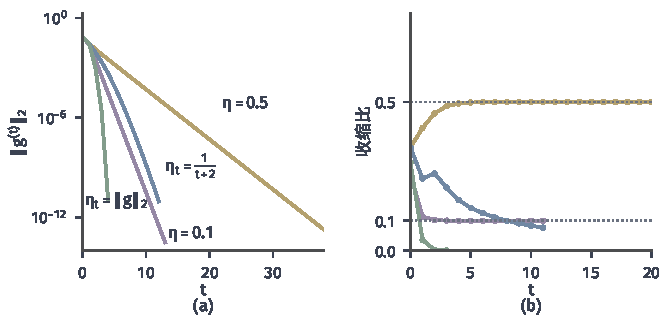
\includegraphics[width=112mm]{figures/05-optimization/02-smooth-optimization/matplotlib/newton-eta-rates/figure.pdf}
  \caption{误差比例对局部速度的影响，从$(0.9,0.8)$出发，残差取$\eta_t\bm{g}^{(t)}$。(a)梯度范数：黄线$\eta=0.5$、紫线$\eta=0.1$是直线，蓝线$\eta_t=1/(t+2)$越来越陡，绿线$\eta_t=\lVert\bm{g}^{(t)}\rVert_2$几步到底。(b)各线的收缩比$\lVert\bm{A}\bm{e}^{(t+1)}\rVert_2/\lVert\bm{A}\bm{e}^{(t)}\rVert_2$，灰色点线标出$0.5$和$0.1$。}
  \label{fig:newton-eta-rates}
\end{BookInlineFigure}

\paragraph{远离解时}
局部定理只说解附近。在远处，条件~\eqref{eq:newton-inexact-condition}本身甚至不保证方向下降。把$\bm{d}=\bm{H}^{-1}(\bm{r}-\bm{g})$代入方向导数，得到
\[
 \bm{g}^\top\bm{d}=-\bm{g}^\top\bm{H}^{-1}\bm{g}+\bm{g}^\top\bm{H}^{-1}\bm{r}.
\]
第二项的大小可以超过第一项。设$\bm{H}$正定，比较两项的界，能够保证方向导数为负的充分条件是$\eta_t<1/\kappa(\bm{H})$，这在病态时非常苛刻。

具体的例子如下。取
\[
 \bm{H}=\operatorname{diag}(1,100),\qquad \bm{g}=(1,10).
\]
Newton方向是$\bm{d}_{\mathrm{N}}=(-1,-0.1)$。取残差$\bm{r}=(2.5,0.25)$，比例为
\[
 \frac{\lVert\bm{r}\rVert_2}{\lVert\bm{g}\rVert_2}=\frac{2.5125}{10.050}=0.25.
\]
对应的方向是
\[
 \bm{d}=\bm{H}^{-1}(\bm{r}-\bm{g})=(1.5,-0.0975).
\]
它的方向导数是$\bm{g}^\top\bm{d}=1.5-0.975=0.525>0$，满足残差条件，却是上坡方向。

图~\ref{fig:newton-residual-ellipse}说明了原因。满足条件的方向构成以$\bm{d}_{\mathrm{N}}$为中心的椭球，半轴长度正比于$\eta\lVert\bm{g}\rVert_2/\lambda_i$。Hessian的小特征值方向上半轴很长，椭球可以越过$\bm{g}^\top\bm{d}=0$的分界面。

\begin{BookInlineFigure}
  \centering
  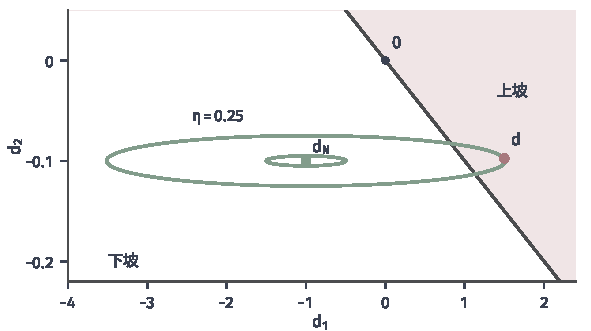
\includegraphics[width=100mm]{figures/05-optimization/02-smooth-optimization/matplotlib/newton-residual-ellipse/figure.pdf}
  \caption{方向空间中满足残差条件的集合，$\bm{H}=\operatorname{diag}(1,100)$，$\bm{g}=(1,10)$，注意两轴比例不同。绿色椭圆分别是$\eta=0.25$和$\eta=0.05$的边界，绿点是Newton方向，深灰色粗线是$\bm{g}^\top\bm{d}=0$，红色浅底是上坡方向的区域。红点$\bm{d}$的残差比例为$0.25$，却落在上坡区域内。}
  \label{fig:newton-residual-ellipse}
\end{BookInlineFigure}

因此远离解时还需要两样东西：内层算法要能保证给出下降方向，外层仍然要作线搜索。一般的迭代线性求解器并不提供前者，下一小节的共轭梯度法却恰好能提供。

\subsection{Newton-CG}
\label{sec:newton-cg}

\paragraph{主要思想}
Newton方程的系数矩阵对称，在解附近还正定，最自然的内层算法是共轭梯度法，这种组合称为\term{Newton-CG}（Newton conjugate gradient method）。它的吸引力在于，内层只需要能计算$\bm{H}^{(t)}$乘向量，完全不必形成矩阵。

共轭梯度法的完整推导可参考\BookChapterRef{chap:krylov-methods}{卷二第15章“Krylov子空间法”}，这里只复述用到的结论。为了和式~\eqref{eq:newton-residual}保持一致，把残差定义成$\bm{r}_j=\bm{H}\bm{z}_j+\bm{g}$。从$\bm{z}_0=\bm{0}$，$\bm{r}_0=\bm{g}$，$\bm{p}_0=-\bm{g}$出发，第$j$步计算
\begin{equation}
 \alpha_j=\frac{\bm{r}_j^\top\bm{r}_j}{\bm{p}_j^\top\bm{H}\bm{p}_j},\qquad
 \bm{z}_{j+1}=\bm{z}_j+\alpha_j\bm{p}_j,\qquad
 \bm{r}_{j+1}=\bm{r}_j+\alpha_j\bm{H}\bm{p}_j,
 \label{eq:newton-cg-step}
\end{equation}
\begin{equation}
 \beta_{j}=\frac{\bm{r}_{j+1}^\top\bm{r}_{j+1}}{\bm{r}_j^\top\bm{r}_j},\qquad
 \bm{p}_{j+1}=-\bm{r}_{j+1}+\beta_j\bm{p}_j.
 \label{eq:newton-cg-direction}
\end{equation}
这里$\alpha_j$沿$\bm{p}_j$精确极小化模型，每步新的残差与之前的方向正交，新的方向与之前的方向关于$\bm{H}$共轭。

\paragraph{Hessian向量积}
式~\eqref{eq:newton-cg-step}中对$\bm{H}$的唯一需求是计算乘积$\bm{H}\bm{v}$，称为\term{Hessian向量积}（Hessian-vector product）。它是梯度沿$\bm{v}$的方向导数，所以有三种取得的办法。

第一种是直接公式。对目标~\eqref{eq:newton-running-objective}，由式~\eqref{eq:newton-running-derivatives}，
\[
 \bm{H}\bm{v}=\begin{bmatrix}(1-4u+8x_1^2)v_1-4x_1v_2\\-4x_1v_1+2v_2\end{bmatrix}.
\]
只用几次标量运算，不需要存矩阵。

第二种是差分近似，只调用两次梯度：
\begin{equation}
 \bm{H}\bm{v}\approx\frac{\nabla f(\bm{x}+h\bm{v})-\nabla f(\bm{x})}{h}.
 \label{eq:newton-hvp-difference}
\end{equation}
误差约与$h$成正比。$h$太小时舍入误差又会放大，通常取$h$约为机器精度的平方根除以$\lVert\bm{v}\rVert_2$的量级。

第三种是自动微分，可以精确得到$\bm{H}\bm{v}$，代价是梯度计算的常数倍。无论哪一种，一次乘积的成本都与一次梯度同量级。

\paragraph{CG产生的方向总是下降的}
共轭梯度法有一个一般线性求解器没有的性质：只要迄今各步的曲率都为正，它的每个迭代$\bm{z}_j$（$j\geq1$）都是下降方向，而且这一点不依赖$\eta_t$。

\begin{lemma}[CG迭代的下降性]
\label{lem:newton-cg-descent}
设$\bm{g}\neq\bm{0}$，CG运行到第$j\geq1$步，且$\bm{p}_i^\top\bm{H}\bm{p}_i>0$（$i<j$）。则
\begin{equation}
 \bm{g}^\top\bm{z}_j=-\sum_{i=0}^{j-1}\alpha_i\bm{r}_i^\top\bm{r}_i<0.
 \label{eq:newton-cg-descent}
\end{equation}
\end{lemma}

\begin{proof}
由$\bm{z}_j=\sum_{i<j}\alpha_i\bm{p}_i$，只需计算$\bm{g}^\top\bm{p}_i$。残差的递推给出$\bm{r}_i=\bm{g}+\bm{H}\sum_{k<i}\alpha_k\bm{p}_k$，而$\bm{p}_i$与之前的方向关于$\bm{H}$共轭，所以
\[
 \bm{g}^\top\bm{p}_i=\bm{r}_i^\top\bm{p}_i.
\]
再由式~\eqref{eq:newton-cg-direction}和$\bm{r}_i$与$\bm{p}_{i-1}$正交，
\[
 \bm{r}_i^\top\bm{p}_i=-\bm{r}_i^\top\bm{r}_i.
\]
上述正交和共轭关系只依赖算法的代数恒等式，在各步曲率非零时成立，不需要$\bm{H}$整体正定。代回去，再由$\alpha_i>0$和$\bm{r}_0=\bm{g}\neq\bm{0}$，即得结论。
\end{proof}

\paragraph{遇到非正曲率}
在式~\eqref{eq:newton-cg-step}中，$\bm{p}_j^\top\bm{H}\bm{p}_j\leq0$说明$\bm{H}$不是正定的，模型沿这个方向无下界，$\alpha_j$的公式失去意义。此时内层必须结束。常用的规则是，给定很小的$\epsilon\geq0$，当曲率不超过$\epsilon\lVert\bm{p}_j\rVert_2^2$时：
\begin{equation}
 \bm{d}^{(t)}=\begin{cases}-\bm{g}^{(t)},&j=0,\\\bm{z}_j,&j\geq1.\end{cases}
 \label{eq:newton-cg-truncate}
\end{equation}
第一种情形没有已完成的进展，就退回负梯度。第二种情形返回当前的$\bm{z}_j$，由引理~\ref{lem:newton-cg-descent}，它是下降方向。

图~\ref{fig:newton-cg-truncation}把两种情况放在一起。图(a)在点$(\tfrac12,0)$处，模型是碗，CG两步到达Newton方向。具体来说，此处$\bm{g}=(0,-\tfrac12)$，第一步的方向和乘积是
\[
 \bm{p}_0=\bigl(0,\tfrac12\bigr),\qquad \bm{H}\bm{p}_0=(-1,1).
\]
曲率为$\tfrac12$，步长$\alpha_0=\tfrac12$，第一步得到
\[
 \bm{z}_1=\bigl(0,\tfrac14\bigr),\qquad \bm{r}_1=\bigl(-\tfrac12,0\bigr).
\]
第二步$\beta_0=1$，方向和乘积是
\[
 \bm{p}_1=\bigl(\tfrac12,\tfrac12\bigr),\qquad \bm{H}\bm{p}_1=(1,0).
\]
曲率仍为$\tfrac12$，步长$\alpha_1=\tfrac12$，于是
\[
 \bm{z}_2=\bigl(\tfrac14,\tfrac12\bigr),\qquad \bm{r}_2=\bm{0}.
\]
这正好是第~\ref{sec:newton-basic}节算过的Newton方向。

\begin{BookInlineFigure}
  \centering
  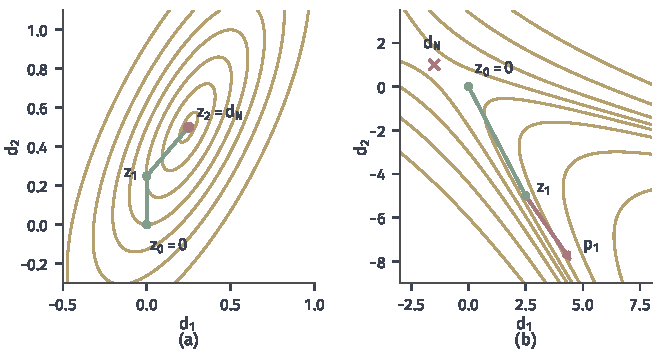
\includegraphics[width=112mm]{figures/05-optimization/02-smooth-optimization/matplotlib/newton-cg-truncation/figure.pdf}
  \caption{位移空间中的内层共轭梯度，黄线是局部模型的等高线。(a)在$(\tfrac12,0)$处模型是碗，绿色折线两步到达红点所示的Newton方向。(b)在$(-\tfrac12,\tfrac34)$处模型不定，绿线是第一步，红色箭头$\bm{p}_1$（按$0.05$倍绘制）是遇到的负曲率方向，内层在$\bm{z}_1$处停止；红叉是Newton方程的解，它是模型的鞍点。}
  \label{fig:newton-cg-truncation}
\end{BookInlineFigure}

\paragraph{与非线性共轭梯度的区别}
第~\ref{chap:first-order-methods}章的非线性共轭梯度法也叫共轭梯度，两者在做不同的事。

\begin{BookInlineTable}
  \centering
  \begin{tabular}{@{}lll@{}}
    \toprule
    & Newton-CG的内层 & 非线性共轭梯度法 \\
    \midrule
    作用对象 & 固定的二次模型 & 原目标 \\
    每步信息 & 一次$\bm{H}\bm{v}$ & 梯度和线搜索的函数值 \\
    步长 & 式~\eqref{eq:newton-cg-step}的闭式公式 & 线搜索 \\
    共轭性 & 模型上精确（不计舍入） & 一般只近似成立 \\
    有限步终止 & 不超过$n$步 & 没有此结论 \\
    \bottomrule
  \end{tabular}
  \caption{二次模型上的线性共轭梯度和直接作用于原目标的非线性共轭梯度。前者是一轮外层迭代中的线性方程求解器。}
  \label{tab:newton-cg-vs-ncg}
\end{BookInlineTable}

\paragraph{计算过程}
外层和内层的关系见图~\ref{fig:newton-cg-loops}。下面用目标~\eqref{eq:newton-running-objective}从Hessian不定的点$(-\tfrac12,\tfrac34)$出发。

\begin{BookInlineFigure}
  \centering
  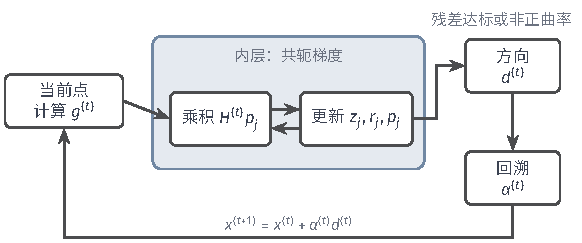
\includegraphics[width=99mm]{figures/05-optimization/02-smooth-optimization/tikz/newton-cg-loops/figure.pdf}
  \caption{Newton-CG的结构。外层读取梯度，内层只通过Hessian向量积与目标交互，在残差达到式~\eqref{eq:newton-inexact-condition}或遇到非正曲率时返回方向$\bm{d}^{(t)}$，外层再用回溯确定步长。}
  \label{fig:newton-cg-loops}
\end{BookInlineFigure}

\needspace{6\baselineskip}
\paragraph{变量}
\begin{itemize}
 \item $\bm{x},\bm{g}$：外层的当前点和梯度。
 \item $\eta_t$：本轮的误差比例。
 \item $\bm{z},\bm{r},\bm{p}$：内层的近似解、残差和搜索方向，每轮外层重新初始化。
 \item $\bm{q}$：工作向量，存放$\bm{H}\bm{p}$。
 \item $\bm{d},\alpha$：外层方向和步长。
 \item 不需要$\bm{H}$的存储，只需要计算$\bm{H}\bm{v}$的子程序。
\end{itemize}

\paragraph{初始化}
选定$\bm{x}^{(0)}$，$c$，$\beta$，$\varepsilon$。例中初始点和外层容差为
\[
 \bm{x}^{(0)}=\bigl(-\tfrac12,\tfrac34\bigr),\qquad c=0.1,\qquad \beta=0.5,\qquad \varepsilon=10^{-6}.
\]
误差比例取式~\eqref{eq:newton-forcing-rule}中的第一种，曲率阈值取$\epsilon=0$。

\needspace{6\baselineskip}
\paragraph{每轮更新}
在第$t$轮外层：
\begin{enumerate}
 \item \textbf{读取梯度并检查停止。}计算$\bm{g}^{(t)}$；若$\lVert\bm{g}^{(t)}\rVert_2\leq\varepsilon$，结束。然后确定$\eta_t$。

 例中第一轮$\bm{g}^{(0)}=(-\tfrac12,1)$，$\lVert\bm{g}^{(0)}\rVert_2=1.118$，$\eta_0=0.5$。

 \item \textbf{内层初始化。}令$\bm{z}_0=\bm{0}$，$\bm{r}_0=\bm{g}^{(t)}$，$\bm{p}_0=-\bm{g}^{(t)}$，$j=0$。

 \item \textbf{内层迭代。}计算$\bm{q}=\bm{H}^{(t)}\bm{p}_j$及曲率$\bm{p}_j^\top\bm{q}$。曲率不超过阈值时按式~\eqref{eq:newton-cg-truncate}返回方向。否则按式~\eqref{eq:newton-cg-step}更新；若$\bm{z}_{j+1}$已满足条件~\eqref{eq:newton-inexact-condition}，就返回它。否则按式~\eqref{eq:newton-cg-direction}更新方向，令$j\leftarrow j+1$。

 例中第一轮外层的第一步内层，$\bm{p}_0=(\tfrac12,-1)$，乘积和曲率为
 \[
  \bm{q}=\begin{bmatrix}-1.5\\-1\end{bmatrix},\qquad \bm{p}_0^\top\bm{q}=0.25>0.
 \]
 步长$\alpha_0=1.25/0.25=5$，更新后
 \[
  \bm{z}_1=\begin{bmatrix}2.5\\-5\end{bmatrix},\qquad \bm{r}_1=\begin{bmatrix}-8\\-4\end{bmatrix}.
 \]
 残差比例是$8.94/1.118=8$，大于$\eta_0$，继续。这个比例大于$1$，说明模型并不是碗。

 第二步内层，$\beta_0=80/1.25=64$，方向、乘积和曲率为
 \[
  \bm{p}_1=\begin{bmatrix}40\\-60\end{bmatrix},\qquad
  \bm{q}=\begin{bmatrix}-80\\-40\end{bmatrix},\qquad
  \bm{p}_1^\top\bm{q}=-800<0.
 \]
 遇到负曲率，由式~\eqref{eq:newton-cg-truncate}返回$\bm{d}^{(0)}=\bm{z}_1=(2.5,-5)$，内层用了$2$次Hessian向量积。

 \item \textbf{回溯并更新。}从$\alpha=1$开始按式~\eqref{eq:newton-armijo}回溯，然后更新$\bm{x}$，令$t\leftarrow t+1$。

 例中第一轮方向导数为$-6.25$。$\alpha=1$和$\tfrac12$的目标值分别是$68.56$和$5.379$，都被拒绝。$\alpha=\tfrac14$的新点是$(0.125,-0.5)$，目标值$0.6487$，低于右端$1.2188$，接受。

 第二轮$\bm{g}^{(1)}=(-0.6172,-1.0313)$，$\lVert\bm{g}^{(1)}\rVert_2=1.202$，$\eta_1=0.5$，Hessian为
 \[
  \bm{H}^{(1)}=\begin{bmatrix}3.1875&-0.5\\-0.5&2\end{bmatrix}.
 \]
 内层第一步的曲率是$2.7047$，$\alpha_0=1.4444/2.7047=0.5340$，于是
 \[
  \bm{z}_1=\begin{bmatrix}0.3296\\0.5507\end{bmatrix},\qquad \bm{r}_1=\begin{bmatrix}0.1581\\-0.0946\end{bmatrix}.
 \]
 残差比例$0.184/1.202=0.153\leq0.5$，内层结束，只用了一次乘积。完整步被接受。
\end{enumerate}

各轮结果见表~\ref{tab:newton-cg-run}。第$9$轮梯度范数低于容差，迭代结束，最终得到$\bm{x}^{(9)}\approx(1,1)$，整个过程用了$14$次Hessian向量积。可以看到比例收紧之前内层大多只走一步，$\eta_t$变小后内层把方程解到精确。

\begin{BookInlineTable}
  \centering
  \begin{tabular}{@{}ccccccc@{}}
    \toprule
    $t$ & $\bm{x}^{(t)}$ & $f$ & $\lVert\bm{g}^{(t)}\rVert_2$ & $\eta_t$ & $\bm{H}\bm{v}$次数 & $\alpha^{(t)}$ \\
    \midrule
    $0$ & $(-0.5,0.75)$ & $1.375$ & $1.118$ & $0.5$ & $2$（负曲率）& $1/4$ \\
    $1$ & $(0.125,-0.5)$ & $0.6487$ & $1.202$ & $0.5$ & $1$ & $1$ \\
    $2$ & $(0.4546,0.0507)$ & $0.1730$ & $0.407$ & $0.5$ & $1$ & $1$ \\
    $3$ & $(0.8099,0.4739)$ & $0.05121$ & $0.540$ & $0.5$ & $1$ & $1$ \\
    $4$ & $(0.7596,0.5197)$ & $0.03218$ & $0.132$ & $0.364$ & $2$ & $1$ \\
    $5$ & $(0.9552,0.8741)$ & $2.47\mathrm{e}{-3}$ & $0.127$ & $0.356$ & $1$ & $1$ \\
    $6$ & $(0.9448,0.8820)$ & $1.64\mathrm{e}{-3}$ & $0.0260$ & $0.161$ & $2$ & $1$ \\
    $7$ & $(0.9977,0.9927)$ & $1.04\mathrm{e}{-5}$ & $0.0105$ & $0.102$ & $2$ & $1$ \\
    $8$ & $(0.99998,0.99995)$ & $3.43\mathrm{e}{-10}$ & $1.13\mathrm{e}{-5}$ & $0.0034$ & $2$ & $1$ \\
    $9$ & $(1.0000,1.0000)$ & & $2.4\mathrm{e}{-9}$ & 停止 & & \\
    \bottomrule
  \end{tabular}
  \caption{Newton-CG在目标~\eqref{eq:newton-running-objective}上的运行，$\eta_t=\min\{0.5,\sqrt{\lVert\bm{g}^{(t)}\rVert_2}\}$。第$0$轮内层因负曲率提前结束。}
  \label{tab:newton-cg-run}
\end{BookInlineTable}

\paragraph{适用范围与补充}
非正曲率规则只保证方向可用，没有利用负曲率本身携带的信息。把遇到的$\bm{p}_j$当作离开鞍点的方向，或者在一个有限半径的区域内求解模型，分别是第~\ref{chap:saddle-points}章和第~\ref{chap:trust-region}章的内容。另外，CG只能看到由$\bm{g}^{(t)}$生成的Krylov子空间；若$\bm{g}^{(t)}$恰好与某个负曲率方向正交，CG也察觉不到它。

Hessian病态时，内层CG本身收敛很慢，这时可以预条件，做法与线性方程中的预条件共轭梯度法相同，见前面引用的Krylov一章。
